% !TEX root = ../Preparazione alle olimpiadi.tex

\chapter{Programmazione Dinamica}

La \textbf{programmazione dinamica} è una particolare tecnica di programmazione che consente di trovare la soluzione a un problema scomponendolo in sottoproblemi più semplici, spesso sovrapposti tra loro, le cui soluzioni vengono memorizzate e riutilizzate per evitare calcoli ripetuti.

Questa tecnica può essere applicata quando un problema presenta una \textit{struttura di sottoproblemi ottimali} e quando i sottoproblemi non sono indipendenti, ma condividono parti comuni.

In questo modo, la programmazione dinamica combina la correttezza della ricerca esaustiva con l’efficienza di un approccio basato sulla memorizzazione dei risultati intermedi.

La programmazione dinamica può essere implementata secondo due approcci principali:

\begin{itemize}
	\item \textbf{Approccio ricorsivo (top-down)}: il problema viene risolto mediante una definizione ricorsiva, calcolando i sottoproblemi solo quando necessari. I risultati ottenuti vengono memorizzati (tecnica di \textit{memoization}) per evitare ricalcoli successivi degli stessi sottoproblemi.
	
	\item \textbf{Approccio iterativo (bottom-up)}: il problema viene risolto partendo dai casi base e costruendo progressivamente la soluzione del problema principale in modo iterativo, memorizzando i risultati intermedi in una struttura dati (ad esempio un array o una tabella), senza ricorrere alla ricorsione.
\end{itemize}

Esistono due principali utilizzi di questa tecnica:
\begin{itemize}
	\item \textbf{Trovare una soluzione ottimale}: si vuole determinare una soluzione che sia massima o minima rispetto a un certo criterio (ad esempio il costo minimo o il guadagno massimo).
	\item \textbf{Contare il numero di soluzioni}: si vuole calcolare il numero totale di soluzioni possibili che soddisfano determinate condizioni.
\end{itemize}

Poiché una trattazione puramente teorica della programmazione dinamica risulta poco intuitiva, è utile introdurre la tecnica attraverso semplici problemi esemplificativi, che ne chiariscono i principi fondamentali.




\section{Programmazione dinamica ricorsiva}


\subsection{Problema del bagno}

Supponiamo di avere un bagno di dimensioni \(1 \times N\) che deve essere piastrellato utilizzando esclusivamente piastrelle di dimensione \(1 \times 1\) e \(1 \times 2\). La situazione è illustrata in Figura \ref{fig:6 - programmazione-dinamica:ricorsiva:bagno}.

\begin{figure}[h!]
	\centering
	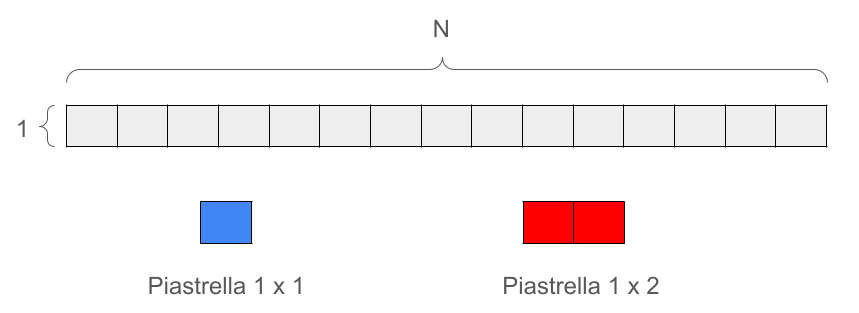
\includegraphics[width=0.8\textwidth]{immagini/6 - Programmazione dinamica/Programmazione dinamica ricorsiva/bagno.png}
	\caption{Rappresentazione del bagno da piastrellare con le piastrelle da utilizzare.}
	\label{fig:6 - programmazione-dinamica:ricorsiva:bagno}
\end{figure}

Ci poniamo la seguente domanda:  
\texttt{quanti modi diversi esistono per completare la piastrellatura combinando le piastrelle disponibili?}


È possibile rispondere immediatamente nel caso in cui le dimensioni del bagno siano \(1 \times 3\). In tale situazione, infatti, i possibili modi di disporre le piastrelle sono:

\begin{itemize}
	\item una piastrella \(1\times1\) seguita da una \(1\times2\);
	\item una piastrella \(1\times2\) seguita da una \(1\times1\);
	\item tre piastrelle \(1\times1\).
\end{itemize}

Pertanto, i modi totali di piastrellare un bagno di dimensione \(1 \times 3\) sono pari a 3 (come mostrato in Figura \ref{fig:6 - programmazione-dinamica:ricorsiva:bagno1x3}).

\begin{figure}[h!]
	\centering
	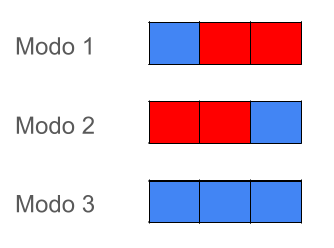
\includegraphics[width=0.5\textwidth]{immagini/6 - Programmazione dinamica/Programmazione dinamica ricorsiva/bagno1x3.png}
	\caption{Modo 1: una piastrella $1\times1$ e una $1\times2$; Modo 2: una piastrella $1\times2$ e una $1\times1$; Modo 3: tre piastrelle $1\times1$}
	\label{fig:6 - programmazione-dinamica:ricorsiva:bagno1x3}
\end{figure}

Il problema diventa meno immediato quando la lunghezza del bagno cresce, ad esempio nei casi \(1 \times 10\) o \(1 \times 1000\), per i quali un’elencazione diretta di tutte le configurazioni risulta impraticabile.

\medskip

Per semplificare la trattazione, introduciamo una quantità \(F(N)\), che rappresenta il numero totale di modi in cui è possibile piastrellare un bagno di dimensione \(1 \times N\). È facile osservare che tale quantità dipende unicamente dalla lunghezza \(N\) della stanza.

Partendo dalla quantità \(F(N)\), possiamo osservare che essa è data dalla somma del numero di modi in cui è possibile piastrellare un bagno di dimensione \(1 \times N\) iniziando con una piastrella \(1 \times 1\) e del numero di modi in cui è possibile piastrellare lo stesso bagno iniziando con una piastrella \(1 \times 2\).

\begin{equation}
	F(N) = F(N-1) + F(N-2)
	\label{eq:ricorrenza_base}
\end{equation}

dove:
\begin{itemize}
	\item \(F(N)\) rappresenta il numero totale di modi per piastrellare un bagno di dimensione \(1 \times N\);
	\item \(F(N-1)\) rappresenta il numero di modi per piastrellare un bagno di dimensione \(1 \times (N-1)\), corrispondente ai casi in cui la prima piastrella è di tipo \(1 \times 1\);
	\item \(F(N-2)\) rappresenta il numero di modi per piastrellare un bagno di dimensione \(1 \times (N-2)\), corrispondente ai casi in cui la prima piastrella è di tipo \(1 \times 2\).
\end{itemize}

Possiamo ora applicare la stessa relazione di ricorrenza \eqref{eq:ricorrenza_base} ai termini \(F(N-1)\) e \(F(N-2)\). In particolare, si ha:

\begin{equation}
	F(N-1) = F(N-2) + F(N-3)
	\label{eq:ricorrenza_FNmeno1}
\end{equation}

\begin{equation}
	F(N-2) = F(N-3) + F(N-4)
	\label{eq:ricorrenza_FNmeno2}
\end{equation}

Sostituendo la \eqref{eq:ricorrenza_FNmeno1} e la \eqref{eq:ricorrenza_FNmeno2} nella \eqref{eq:ricorrenza_base}, otteniamo:

\begin{equation}
	F(N) = F(N-2) + F(N-3) + F(N-3) + F(N-4)
	\label{eq:sviluppo_FN}
\end{equation}

Possiamo osservare come ciascun termine presente nella relazione \eqref{eq:ricorrenza_base} generi due sottotermini, i quali a loro volta ne generano altri due ciascuno, e così via, in modo ricorsivo.  
Ovviamente, non possiamo continuare all'infinito, poiché il bagno ha dimensioni finite. Per questo motivo, è necessario definire dei \textbf{casi base}, che rappresentano le condizioni di \texttt{stop} per la scomposizione ricorsiva.

In particolare, possiamo affermare che:
\begin{itemize}
	\item $F(2) = 2$, corrispondente a due possibili configurazioni: una piastrella $1 \times 2$ oppure due piastrelle $1\times 1$;
	\item $F(1) = 1$, corrispondente a un'unica piastrella $1 \times 1$.
\end{itemize}

Pertanto, i casi base della ricorrenza sono:

\[
F(1) = 1, \quad F(2) = 2.
\]


La struttura che si viene a generare da queste "scomposizioni" è rappresentata in Figura \ref{fig:6 - programmazione-dinamica:ricorsiva:albero}.

\begin{figure}[h!]
	\centering
	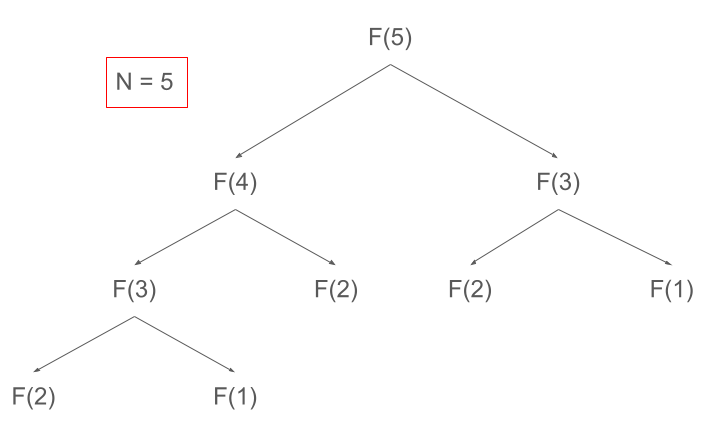
\includegraphics[width=1\textwidth]{immagini/6 - Programmazione dinamica/Programmazione dinamica ricorsiva/albero.png}
	\caption{Albero generato dalla scomposizione dei vari termini supponendo un bagno iniziale di dimensioni $1 \times 5$}
	\label{fig:6 - programmazione-dinamica:ricorsiva:albero}
\end{figure}

Ogni chiamata ricorsiva genera due ulteriori chiamate, dando origine a un albero di ricorsione binario. Di conseguenza, la complessità complessiva dell’algoritmo può essere stimata come \(O(2^N)\).

Per valori elevati di \(N\), tale approccio risulta inefficiente a causa del numero elevato di chiamate ridondanti.  
Osservando la Figura \ref{fig:6 - programmazione-dinamica:ricorsiva:albero}, si nota infatti che i termini presenti nel ramo destro dell’albero di ricorsione, come \(F(3)\), \(F(2)\) e \(F(1)\), sono già stati calcolati nel ramo sinistro.

Pertanto, il ramo destro dell’albero non introduce nuove computazioni utili, ma ripete risultati già ottenuti.  
Evitando di ricalcolare tali termini e memorizzando i valori intermedi, è possibile ridurre la complessità dell’algoritmo da esponenziale a lineare, passando da $2^N$ computazioni a sole $N$ computazioni.
In altre parole, ci basta scendere lungo un solo ramo dell'albero (sinistro) per ottenere tutti i termini di cui abbiamo bisogno.

Il problema è completamente definito attraverso il sistema \eqref{sistema-bagno}.

\begin{equation}
	f(x) =
	\left\{
	\begin{aligned}
		& f(x-1) + f(x-2), && x > 2\\
		& 2, && x = 2\\
		& 1, && x = 1
	\end{aligned}
	\right.
	\label{sistema-bagno}
\end{equation}



\noindent \textbf{Complessità Computazionale:} \\
La complessità computazionale di questo problema, assumendo di non ricalcolare più volte gli stessi sottoproblemi grazie alla memorizzazione dei risultati intermedi, può essere valutata considerando due fattori:

\begin{itemize}
	\item il numero di \textbf{stati distinti}, dove per stati si intendono i sottoproblemi unici da risolvere (corrispondenti alle "foglie" o ai nodi dell'albero di ricorsione);
	\item il \textbf{costo dello stato}, ovvero il tempo necessario per calcolare lo stato corrente a partire dai valori dei sottoproblemi già risolti.
\end{itemize}

Nel caso del problema della piastrellatura del bagno, ogni stato è rappresentato dal numero di modi per piastrellare un bagno di dimensione \(1 \times x\), ossia \(F(x)\), e la transizione di stato consiste semplicemente nella somma di due valori precedenti:

\[
F(x) = F(x-1) + F(x-2)
\]

Poiché il numero di stati distinti è \(N\) e il costo per calcolare ciascun stato è costante (\(O(1)\)), la complessità complessiva dell’algoritmo risulta pari a \(O(N)\).  
In altre parole, ogni sottoproblema viene calcolato una sola volta e tutti i risultati intermedi vengono riutilizzati senza ricalcolo.



\subsection{Problema della griglia}
Supponiamo di avere una griglia con \(N\) righe e \(M\) colonne.  

La posizione di partenza è fissata nella cella in alto a sinistra, \((0,0)\), e l’obiettivo è raggiungere la cella in basso a destra, \((N-1, M-1)\), seguendo la regola "posso muovermi solo in basso o a destra".

L’obiettivo è quindi calcolare il numero di percorsi validi che portano dalla cella iniziale a quella finale rispettando le restrizioni sopra indicate.
La situazione è illustrata graficamente in Figura \ref{fig:6 - programmazione-dinamica:ricorsiva:griglia}


\begin{figure}[h!]
	\centering
	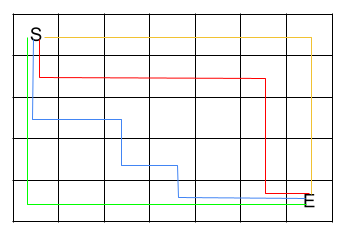
\includegraphics[width=0.7\textwidth]{immagini/6 - Programmazione dinamica/Programmazione dinamica ricorsiva/griglia.png}
	\caption{Illustrazione grafica del problema della griglia.  
		Con \(S\) è indicato il punto di partenza e con \(E\) il punto di arrivo.  
		Sono riportati alcuni dei percorsi possibili che rispettano le regole del movimento (solo verso destra o verso il basso).}
	\label{fig:6 - programmazione-dinamica:ricorsiva:griglia}
\end{figure}

Introduciamo quindi la funzione $f$ che risponde alla domanda: qual è il numero di modi con cui posso arrivare alla cella $E$ a partire dalla mia posizione attuale?
In generale, $f$ dipende dalle coordinate in cui mi trovo, ovvero:

\begin{equation*}
	f = f(riga, colonna) = f(r, c)
\end{equation*}

Utilizzando questa notazione e considerando che il punto di partenza ha coordinate \((0, 0)\), la risposta al problema si ottiene valutando \(f(0, 0)\).  

Possiamo affermare che la generica \(f(r, c)\) sarà data dalla somma di \(f(r+1, c)\) e \(f(r, c+1)\), ovvero dalla somma dei modi con cui posso raggiungere \(E\) facendo un passo verso il basso e dei modi con cui posso raggiungere \(E\) facendo un passo verso destra:

\begin{equation}
	f(r, c) = f(r+1, c) + f(r, c+1)
	\label{frc}
\end{equation}

Inoltre, non sono consentiti movimenti che porterebbero fuori dai confini della griglia. I casi base associati a questa condizione sono:

\begin{equation}
	f(N, c) = 0 \quad \text{per tutte le colonne } c \text{ (fuori dalla griglia in basso)}
	\label{fnc}
\end{equation}

\begin{equation}
	f(r, M) = 0 \quad \text{per tutte le righe } r \text{ (fuori dalla griglia a destra)}
	\label{frm}
\end{equation}

Combinando la \eqref{frc} con le condizioni \eqref{fnc} e \eqref{frm}, si ottiene il sistema \eqref{eq:sistema_frc}.

\begin{equation}
	f(r,c) =
	\left\{
	\begin{aligned}
		& f(r+1, c) + f(r, c+1), && 0 \le r < N, \ 0 \le c < M\\
		& 0, && r = N \text{ (fuori dalla griglia in basso)}\\
		& 0, && c = M \text{ (fuori dalla griglia a destra)}
	\end{aligned}
	\right.
	\label{eq:sistema_frc}
\end{equation}


Il problema è quindi completamente definito e, come vedremo nella codifica, la definizione del sistema \eqref{eq:sistema_frc} è sufficiente per ottenere la soluzione.

\bigskip

\noindent \textbf{Complessità Computazionale:}\\
Come nel problema del piastrellamento del bagno, la complessità computazionale si calcola come prodotto tra il numero di stati distinti e il costo per calcolare ciascuno stato:

\begin{equation}
	\text{Complessità totale} = \text{Numero di stati} \cdot \text{complessità per stato} 
	\label{eq:complessità}
\end{equation}

Nel nostro caso:

\begin{itemize}
	\item Il numero di stati è \(O(N \cdot M)\), corrispondente al numero di celle della griglia.  
	\item La complessità per stato è \(O(1)\), perché calcolare \(f(r,c)\) richiede solo la somma di due valori già calcolati (\(f(r+1,c)\) e \(f(r,c+1)\)).  
\end{itemize}

Da cui la complessità totale dell’algoritmo diventa:

\begin{equation}
	\text{Complessità totale} = O(N \cdot M) \cdot O(1) = O(N \cdot M)
\end{equation}


\subsection{Problema della griglia con monete}
Supponiamo di avere una griglia di dimensione $N \times M$, come nel problema precedente.  
In ogni cella $(r, c)$ è presente una quantità di monete $k[r,c]$, dove $r$ e $c$ indicano la riga e la colonna della cella, rispettivamente.

La situazione è illustrata in Figura \ref{fig:6 - programmazione-dinamica:ricorsiva:griglia-monete}.



\begin{figure}[h!]
	\centering
	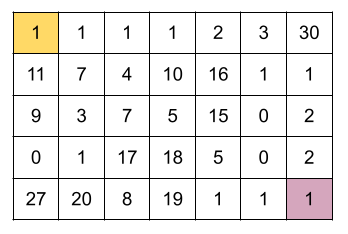
\includegraphics[width=0.7\textwidth]{immagini/6 - Programmazione dinamica/Programmazione dinamica ricorsiva/griglia monete.png}
	\caption{Griglia $N \times M$. In ogni cella è riportata la quantità di monete.}
	\label{fig:6 - programmazione-dinamica:ricorsiva:griglia-monete}
\end{figure}

Partiamo dalla cella di partenza $(0,0)$ (casella gialla) e vogliamo raggiungere la cella finale $(N-1, M-1)$ (casella rosa), muovendoci solo verso destra o verso il basso, e raccogliendo il massimo numero possibile di monete.

Definiamo la funzione $f(r,c)$ come il massimo numero di monete che è possibile raccogliere partendo dalla cella $(r,c)$, rispettando i vincoli del problema.  

Il sistema risolutivo può essere descritto considerando i possibili movimenti dalla cella corrente:

\begin{itemize}
	\item Se mi muovo verso destra, posso raccogliere un numero di monete pari a $f(r, c+1) + k[r,c]$, ovvero il massimo ottenibile dalla cella a destra più le monete presenti nella cella corrente.
	\item Se mi muovo verso il basso, posso raccogliere un numero di monete pari a $f(r+1, c) + k[r,c]$, ovvero il massimo ottenibile dalla cella sottostante più le monete presenti nella cella corrente.
	\item Se mi trovo fuori dai confini della griglia, non posso raccogliere monete: $f(r,c) = 0$.
\end{itemize}

Lo scopo è massimizzare le monete raccolte; pertanto, dalla cella $(r,c)$ sceglierò la direzione che porta al massimo numero di monete.  

Il sistema risultante è, quindi, il seguente:

\begin{equation}
	f(r,c) =
	\left\{
	\begin{aligned}
		& k[r,c] + \max(f(r+1, c), f(r, c+1)), && 0 \le r < N, \ 0 \le c < M\\
		& 0, && r = N \text{ (fuori dalla griglia in basso)}\\
		& 0, && c = M \text{ (fuori dalla griglia a destra)}
	\end{aligned}
	\right.
	\label{eq:sistema_griglia-monete}
\end{equation}

\bigskip
\noindent \textbf{Complessità Computazionale:} \\
Ogni stato della funzione $f(r,c)$ corrisponde a una cella della griglia. Per calcolare il valore di $f(r,c)$ dobbiamo considerare al massimo due transizioni: verso destra o verso il basso.  
Pertanto, la complessità totale dell'algoritmo può essere stimata come:

\begin{equation}
	\text{Complessità totale} = \text{Numero di stati} \cdot \text{Costo per stato} 
	\label{eq:complessita_monete}
\end{equation}

Nel nostro caso:

\begin{itemize}
	\item Il numero di stati è pari a $N \cdot M$, corrispondente al numero di celle della griglia.
	\item Il costo per stato è $O(1)$, perché per ogni cella dobbiamo solo calcolare la somma delle monete della cella corrente e il massimo tra due valori già calcolati.
\end{itemize}

\begin{equation}
	\text{Complessità totale} = O(N \cdot M) \cdot O(1) = O(N \cdot M)
\end{equation}
